\documentclass{standalone}
\usepackage{tikz}
\usetikzlibrary{patterns, positioning}

\begin{document}
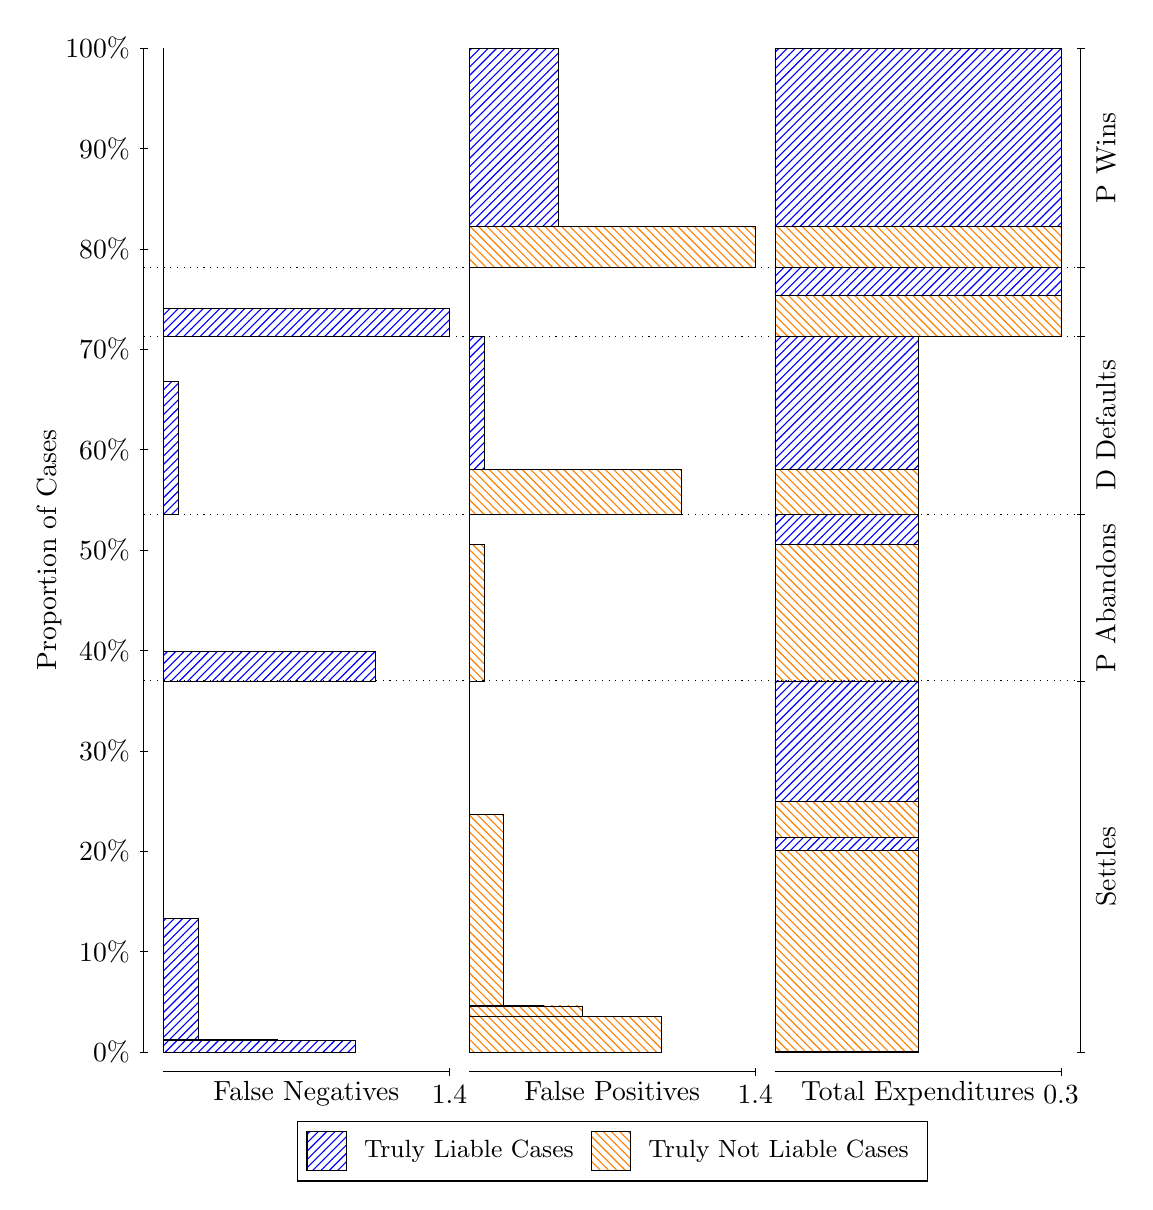
\begin{tikzpicture}
\draw[black, very thin] (1.5,1.75) -- (1.5,14.5);
\node[rotate=90, anchor=center] at (0.3, 8.125) {Proportion of Cases};
\draw[black, very thin] (1.45,1.75) -- (1.55,1.75);
\node[anchor=east] at (1.45, 1.75) {0\%};
\draw[black, very thin] (1.45,3.025) -- (1.55,3.025);
\node[anchor=east] at (1.45, 3.025) {10\%};
\draw[black, very thin] (1.45,4.3) -- (1.55,4.3);
\node[anchor=east] at (1.45, 4.3) {20\%};
\draw[black, very thin] (1.45,5.575) -- (1.55,5.575);
\node[anchor=east] at (1.45, 5.575) {30\%};
\draw[black, very thin] (1.45,6.85) -- (1.55,6.85);
\node[anchor=east] at (1.45, 6.85) {40\%};
\draw[black, very thin] (1.45,8.125) -- (1.55,8.125);
\node[anchor=east] at (1.45, 8.125) {50\%};
\draw[black, very thin] (1.45,9.4) -- (1.55,9.4);
\node[anchor=east] at (1.45, 9.4) {60\%};
\draw[black, very thin] (1.45,10.675) -- (1.55,10.675);
\node[anchor=east] at (1.45, 10.675) {70\%};
\draw[black, very thin] (1.45,11.95) -- (1.55,11.95);
\node[anchor=east] at (1.45, 11.95) {80\%};
\draw[black, very thin] (1.45,13.225) -- (1.55,13.225);
\node[anchor=east] at (1.45, 13.225) {90\%};
\draw[black, very thin] (1.45,14.5) -- (1.55,14.5);
\node[anchor=east] at (1.45, 14.5) {100\%};

\draw[black, very thin] (13.4,1.75) -- (13.4,14.5);
\draw[black, very thin] (13.35,1.75) -- (13.45,1.75);
\node[anchor=west] at (13.35, 1.75) {};
\draw[black, very thin] (13.35,6.4637) -- (13.45,6.4637);
\node[anchor=west] at (13.35, 6.4637) {};
\draw[black, very thin] (13.35,8.574) -- (13.45,8.574);
\node[anchor=west] at (13.35, 8.574) {};
\draw[black, very thin] (13.35,10.84) -- (13.45,10.84);
\node[anchor=west] at (13.35, 10.84) {};
\draw[black, very thin] (13.35,11.713) -- (13.45,11.713);
\node[anchor=west] at (13.35, 11.713) {};
\draw[black, very thin] (13.35,14.5) -- (13.45,14.5);
\node[anchor=west] at (13.35, 14.5) {};

\draw[black, very thin, pattern color=blue, pattern=north east lines] (1.75,1.75) rectangle (4.1931,1.8993);
\draw[black, very thin, pattern color=blue, pattern=north east lines] (1.75,1.8993) rectangle (3.9425,1.8995);
\draw[black, very thin, pattern color=blue, pattern=north east lines] (1.75,1.8995) rectangle (3.692,1.8996);
\draw[black, very thin, pattern color=blue, pattern=north east lines] (1.75,1.8996) rectangle (3.4414,1.8997);
\draw[black, very thin, pattern color=blue, pattern=north east lines] (1.75,1.8997) rectangle (3.1908,1.9097);
\draw[black, very thin, pattern color=blue, pattern=north east lines] (1.75,1.9097) rectangle (2.1885,3.4441);
\draw[black, very thin, pattern color=orange, pattern=north west lines] (1.75,3.4441) rectangle (1.75,6.4637);
\draw[black, very thin, pattern color=blue, pattern=north east lines] (1.75,6.4637) rectangle (4.4437,6.8421);
\draw[black, very thin, pattern color=orange, pattern=north west lines] (1.75,6.8421) rectangle (1.75,8.574);
\draw[black, very thin, pattern color=blue, pattern=north east lines] (1.75,8.574) rectangle (1.9379,10.264);
\draw[black, very thin, pattern color=orange, pattern=north west lines] (1.75,10.264) rectangle (1.75,10.84);
\draw[black, very thin, pattern color=blue, pattern=north east lines] (1.75,10.84) rectangle (5.3833,11.19);
\draw[black, very thin, pattern color=orange, pattern=north west lines] (1.75,11.19) rectangle (1.75,11.713);
\draw[black, very thin, pattern color=orange, pattern=north west lines] (1.75,11.713) rectangle (1.75,12.238);
\draw[black, very thin, pattern color=blue, pattern=north east lines] (1.75,12.238) rectangle (1.75,14.5);
\draw[black, very thin, pattern color=orange, pattern=north west lines] (5.6333,1.75) rectangle (8.0764,2.2052);
\draw[black, very thin, pattern color=orange, pattern=north west lines] (5.6333,2.2052) rectangle (7.0741,2.3343);
\draw[black, very thin, pattern color=orange, pattern=north west lines] (5.6333,2.3343) rectangle (6.8236,2.3358);
\draw[black, very thin, pattern color=orange, pattern=north west lines] (5.6333,2.3358) rectangle (6.573,2.3373);
\draw[black, very thin, pattern color=orange, pattern=north west lines] (5.6333,2.3373) rectangle (6.3224,2.3388);
\draw[black, very thin, pattern color=orange, pattern=north west lines] (5.6333,2.3388) rectangle (6.0718,4.7697);
\draw[black, very thin, pattern color=blue, pattern=north east lines] (5.6333,4.7697) rectangle (5.6333,6.4637);
\draw[black, very thin, pattern color=orange, pattern=north west lines] (5.6333,6.4637) rectangle (5.8213,8.1957);
\draw[black, very thin, pattern color=blue, pattern=north east lines] (5.6333,8.1957) rectangle (5.6333,8.574);
\draw[black, very thin, pattern color=orange, pattern=north west lines] (5.6333,8.574) rectangle (8.327,9.1497);
\draw[black, very thin, pattern color=blue, pattern=north east lines] (5.6333,9.1497) rectangle (5.8213,10.84);
\draw[black, very thin, pattern color=orange, pattern=north west lines] (5.6333,10.84) rectangle (5.6333,11.362);
\draw[black, very thin, pattern color=blue, pattern=north east lines] (5.6333,11.362) rectangle (5.6333,11.713);
\draw[black, very thin, pattern color=orange, pattern=north west lines] (5.6333,11.713) rectangle (9.2667,12.238);
\draw[black, very thin, pattern color=blue, pattern=north east lines] (5.6333,12.238) rectangle (6.7609,14.5);
\draw[black, very thin, pattern color=orange, pattern=north west lines] (9.5167,1.75) rectangle (11.333,1.7546);
\draw[black, very thin, pattern color=blue, pattern=north east lines] (9.5167,1.7546) rectangle (11.333,1.7549);
\draw[black, very thin, pattern color=orange, pattern=north west lines] (9.5167,1.7549) rectangle (11.333,4.3148);
\draw[black, very thin, pattern color=blue, pattern=north east lines] (9.5167,4.3148) rectangle (11.333,4.4742);
\draw[black, very thin, pattern color=orange, pattern=north west lines] (9.5167,4.4742) rectangle (11.333,4.9294);
\draw[black, very thin, pattern color=blue, pattern=north east lines] (9.5167,4.9294) rectangle (11.333,6.4637);
\draw[black, very thin, pattern color=orange, pattern=north west lines] (9.5167,6.4637) rectangle (11.333,8.1957);
\draw[black, very thin, pattern color=blue, pattern=north east lines] (9.5167,8.1957) rectangle (11.333,8.574);
\draw[black, very thin, pattern color=orange, pattern=north west lines] (9.5167,8.574) rectangle (11.333,9.1497);
\draw[black, very thin, pattern color=blue, pattern=north east lines] (9.5167,9.1497) rectangle (11.333,10.84);
\draw[black, very thin, pattern color=orange, pattern=north west lines] (9.5167,10.84) rectangle (13.15,11.362);
\draw[black, very thin, pattern color=blue, pattern=north east lines] (9.5167,11.362) rectangle (13.15,11.713);
\draw[black, very thin, pattern color=orange, pattern=north west lines] (9.5167,11.713) rectangle (13.15,12.238);
\draw[black, very thin, pattern color=blue, pattern=north east lines] (9.5167,12.238) rectangle (13.15,14.5);
\draw[black, dotted] (1.5,6.4637) -- (13.4,6.4637);
\draw[black, dotted] (1.5,8.574) -- (13.4,8.574);
\draw[black, dotted] (1.5,10.84) -- (13.4,10.84);
\draw[black, dotted] (1.5,11.713) -- (13.4,11.713);
\draw[black, very thin] (1.75,1.5) -- (5.3833,1.5);
\node[anchor=north] at (3.5667, 1.5) {False Negatives};
\draw[black, very thin] (5.3833,1.45) -- (5.3833,1.55);
\node[anchor=north] at (5.3833, 1.45) {1.4};

\draw[black, very thin] (5.6333,1.5) -- (9.2667,1.5);
\node[anchor=north] at (7.45, 1.5) {False Positives};
\draw[black, very thin] (9.2667,1.45) -- (9.2667,1.55);
\node[anchor=north] at (9.2667, 1.45) {1.4};

\draw[black, very thin] (9.5167,1.5) -- (13.15,1.5);
\node[anchor=north] at (11.333, 1.5) {Total Expenditures};
\draw[black, very thin] (13.15,1.45) -- (13.15,1.55);
\node[anchor=north] at (13.15, 1.45) {0.3};

\node[black, centered, rotate=90] at (13.72, 4.1069) {Settles};
\node[black, centered, rotate=90] at (13.72, 7.5189) {P Abandons};
\node[black, centered, rotate=90] at (13.72, 9.7068) {D Defaults};

\node[black, centered, rotate=90] at (13.72, 13.106) {P Wins};

\draw (7.449999999999999,1.5) node[draw=none] (baseCoordinate) {};
\begin{scope}[align=center]
        \matrix[scale=0.5, draw=black, below=0.5cm of baseCoordinate, nodes={draw}, column sep=0.1cm]{
            \node[rectangle, draw, minimum width=0.5cm, minimum height=0.5cm, pattern=north east lines, pattern color=blue] {}; &
            \node[draw=none, font=\small] (B) {Truly Liable Cases}; &
            \node[rectangle, draw, minimum width=0.5cm, minimum height=0.5cm, pattern=north west lines, pattern color=orange] {}; &
            \node[draw=none, font=\small] (B) {Truly Not Liable Cases}; \\
            };
\end{scope}

\end{tikzpicture}
\end{document}